\chapter{Opis projektnog zadatka}
				
		Cilj ovog projekta je razviti programsku podršku za oblikovanje web aplikacije \textit{Ozdravi} koja će korisnicima omogućiti lakšu komunikaciju s liječnicima te brži način dolaska do potvrde o bolovanju zbog bolesti djeteta. Glavna ideja je omogućiti interakciju između više instanci u zdravstvu.
		
		Ova aplikacija namijenjena je prvenstveno roditeljima koji imaju djecu podložnu čestim zdravstvenim problemima, ali mogu ju koristiti svi roditelji.\\
		
		Prilikom otvaranja glavne stranice, neregistrirani korisnik može vidjeti opis aplikacije te specifičnosti koje nudi. Omogućeno mu je prijavljivanje u sustav s postojećim računom (prijava s OIB-om i lozinkom) ili kreiranje novog računa. Za kreiranje novog računa su mu također potrebni samo OIB i lozinka koju želi postaviti za svoj račun. Registrirati se mogu samo roditelji, dok su računi liječnika i pedijatra već postojeći u sustavu te se oni samo prijavljuju.\\
		
		Vrste korisnika web aplikacije su:
		\begin{packed_item}
			\item Roditelj
			\item Liječnik obiteljske medicine
			\item Pedijatar
			\item Administrator
			
		\end{packed_item}
		
		
		\textit{Roditelj} prijavom u sustav može odabrati želi li ući u svoj profil ili u profil djeteta. Pri ulasku u profil roditelj ima opciju pregleda pristiglih poruka ili opciju pregleda osobnih podataka profila. Važnu mogućnost koju ima roditelj je dodavanje maila svog poslodavca u sustav (preko svoga profila) te dodavanje maila škole ili vrtića za pojedino dijete (preko profila djeteta). 
		
		Najvažnija funkcionalnost koju pruža aplikacija i po čemu se ona razlikuje od postojećih je mogućnost automatiziranog odobravanja bolovanja. Roditelj će na svom profilu primiti obavijest ako mu je odobreno bolovanje (zbog svoje bolesti ili bolesti djeteta) te informaciju je li o tome obaviješten i poslodavac (preko maila koji je roditelj upisao na profilu). Na profilu djeteta će roditelj primiti obavijest ako je pedijatar potvrdio bolest djeteta te informaciju o tome je li ispričnica poslana vrtiću ili školi.
		
		Osim te funkcionalnosti, roditelj može za sebe ili za dijete učitati nalaz u sustav, pregledati nalaz iz laboratorija kojeg je poslao liječnik ili pedijatar te pregledati pregled na kojem je naručen on ili njegovo dijete (na odgovarajućem profilu). Ovdje je vidljiva i još jedna mogućnost koju nudi aplikacija - roditelju će se prikazati karta gdje će biti označen sve zdravstvene institucije u kojima je moguće obaviti vrstu pregleda za koju je roditelj ili njegovo dijete naručeno.\\
		
		
		\textit{Pedijatar} pri prijavi u sustav ima popis djece prijavljene kod njega te ima opciju prijavljivanja novog djeteta kod sebe. Pri odabiru određenog djeteta mu se otvori prozor gdje može vidjeti povijest poruka s roditeljem djeteta. Pedijatar ima niz mogućnosti kao što su slanje nalaza iz laboratorija ili naručivanje djeteta na specijalistički pregled. 
		
		Glavna mogućnost je unos podataka o obavljenom pregledu tj. dijagnozi djeteta pri čemu pedijatar može odabrati i opciju da se vrtiću/školi šalje ispričnica te zatražiti bolovanje roditelja. Preporuka za bolovanje roditelja će se proslijediti liječniku. Time se roditelj oslobodađa od potrebe za odlaskom i do pedijatra i do liječnika da bi mu se potencijalno odobrilo bolovanje - to se sve automatizira u sustavu.\\
		
		
		\textit{Liječnik obiteljske medicine} pri prijavi u sustav ima pred sobom popis prijavljenih roditelja kod njega te ima opciju prijavljivanja novog roditelja. Pri odabiru određenog pacijenta otvara mu se prozor gdje može vidjeti poruke koje je s njim izmijenio. Liječnik ima niz mogućnosti kao i pedijatar: slanje nalaza iz laboratorija roditelja te naručivanje roditelja na specijalistički pregled. 
		
		U okviru ove aplikacije najvažnija je činjenica da liječnik roditelju preko aplikacije može odobriti bolovanje. Prvi način kojim se to postiže je standardan: liječnik može upisati podatke o obavljenom pregledu i dijagnozi te odabrati opciju "Propisati bolovanje" ako je to nužno. Drugi način je da liječnik odobri preporuku za bolovanje koju je ponudio pedijatar na temelju bolesti djeteta. Potvrđivanjem te preporuke roditelju dolazi poruka o odobrenom bolovanju. \\
		
		
		\textit{Administrator} ima mogućnost upravljanja korisničkim računima roditelja. Administrator je taj koji u sustav upisuje postojeće osobe (njihovo ime, prezime i OIB), a roditelj se može registrirati samo ako u aplikaciji postoji zapis o njegovom postojanju. Administrator u sustav upisuje i djecu već upisanih roditelja koju onda može povezati s njihovim roditeljem unutar sustava - time roditelj dobiva mogućnost pregleda profila tog djeteta prilikom prijave u sustav. Administrator ima mogućnost i mijenjanja osobnih podataka i roditelja i djece.\\
		
		
		Ova web aplikacija može se usporediti s uslugom Portal zdravlja koja je građanima dostupna preko sustava E-Građani. Portal zdravlja nudi neke slične mogućnosti kao i aplikacija \textit{Ozdravi}. Roditelj može pregledavati svoj profil ili profil djeteta. Na profilu može vidjeti nadležnog liječnika, popis prošlih dijagnoza, nalaze iz laboratorija te se može i naručiti ili otkazati pregled.
		 
		Ipak, Portal zdravlja ne nudi važnu opciju koju nudi i ova aplikacija - mogućnost izdavanja bolovanja roditelju na temelju bolesti djeteta bez da pritom roditelj mora ići i do pedijatra, i do liječnika, i do poslodavca. Sustav web aplikacije automatski zahtjev za bolovanjem šalje od pedijatra, do liječnika te naposljetku i do poslodavca, a roditelj je o tome obaviješten preko poruke.\\
		
		\begin{figure}[H]
			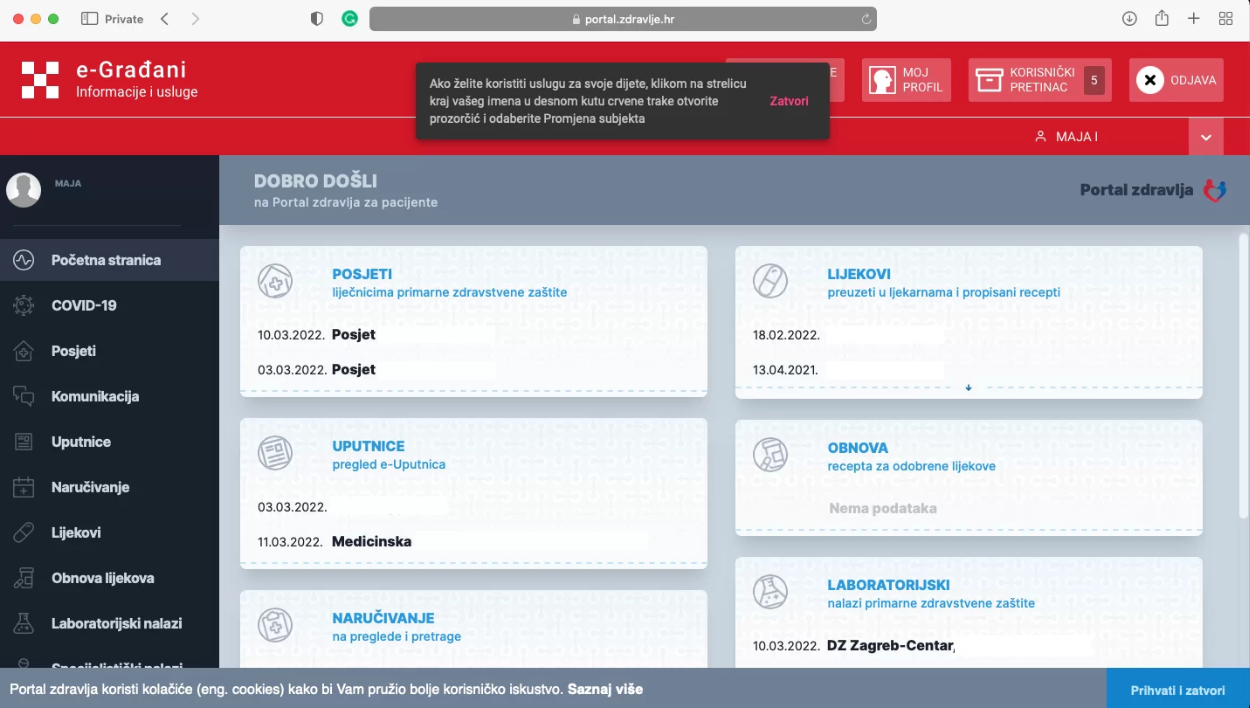
\includegraphics[width=\textwidth]{slike/portalZdravlja.PNG} %veličina u odnosu na širinu linije
			\caption{Snimka zaslona koja prikazuje usluge Portala zdravlja}
		\end{figure}
		
		Sustav bi se u budućnosti mogao nadograditi tako da roditelju dozvoljava mogućnost naručivanja pregleda i biranja termina za sebe i svoju djecu direktno iz aplikacije. Također, sučelje bi se moglo optimizirati time da se poruke mogu filtrirati po vrsti poruke (naručen pregled, nalaz iz laboratorija itd.). Obavljeni pregledi i dijagnoze mogli bi se smjestiti u zasebnom prozoru radi preglednosti. 
		
		\section{Primjeri u \LaTeX u}
		
		\textit{Ovo potpoglavlje izbrisati.}\\

		U nastavku se nalaze različiti primjeri kako koristiti osnovne funkcionalnosti \LaTeX a koje su potrebne za izradu dokumentacije. Za dodatnu pomoć obratiti se asistentu na projektu ili potražiti upute na sljedećim web sjedištima:
		\begin{itemize}
			\item Upute za izradu diplomskog rada u \LaTeX u - \url{https://www.fer.unizg.hr/_download/repository/LaTeX-upute.pdf}
			\item \LaTeX\ projekt - \url{https://www.latex-project.org/help/}
			\item StackExchange za Tex - \url{https://tex.stackexchange.com/}\\
		
		\end{itemize} 	


		
		\noindent \underbar{podcrtani tekst}, \textbf{podebljani tekst}, 	\textit{nagnuti tekst}\\
		\noindent \normalsize primjer \large primjer \Large primjer \LARGE {primjer} \huge {primjer} \Huge primjer \normalsize
				
		\begin{packed_item}
			
			\item  primjer
			\item  primjer
			\item  primjer
			\item[] \begin{packed_enum}
				\item primjer
				\item[] \begin{packed_enum}
					\item[1.a] primjer
					\item[b] primjer
				\end{packed_enum}
				\item primjer
			\end{packed_enum}
			
		\end{packed_item}
		
		\noindent primjer url-a: \url{https://www.fer.unizg.hr/predmet/proinz/projekt}
		
		\noindent posebni znakovi: \# \$ \% \& \{ \} \_ 
		$|$ $<$ $>$ 
		\^{} 
		\~{} 
		$\backslash$ 
		
		
		\begin{longtblr}[
			label=none,
			entry=none
			]{
				width = \textwidth,
				colspec={|X[8,l]|X[8, l]|X[16, l]|}, 
				rowhead = 1,
			} %definicija širine tablice, širine stupaca, poravnanje i broja redaka naslova tablice
			\hline \SetCell[c=3]{c}{\textbf{naslov unutar tablice}}	 \\ \hline[3pt]
			\SetCell{LightGreen}IDKorisnik & INT	&  	Lorem ipsum dolor sit amet, consectetur adipiscing elit, sed do eiusmod  	\\ \hline
			korisnickoIme	& VARCHAR &   	\\ \hline 
			email & VARCHAR &   \\ \hline 
			ime & VARCHAR	&  		\\ \hline 
			\SetCell{LightBlue} primjer	& VARCHAR &   	\\ \hline 
		\end{longtblr}
		

		\begin{longtblr}[
				caption = {Naslov s referencom izvan tablice},
				entry = {Short Caption},
			]{
				width = \textwidth, 
				colspec = {|X[8,l]|X[8,l]|X[16,l]|}, 
				rowhead = 1,
			}
			\hline
			\SetCell{LightGreen}IDKorisnik & INT	&  	Lorem ipsum dolor sit amet, consectetur adipiscing elit, sed do eiusmod  	\\ \hline
			korisnickoIme	& VARCHAR &   	\\ \hline 
			email & VARCHAR &   \\ \hline 
			ime & VARCHAR	&  		\\ \hline 
			\SetCell{LightBlue} primjer	& VARCHAR &   	\\ \hline 
		\end{longtblr}
	


		
		
		%unos slike
		\begin{figure}[H]
			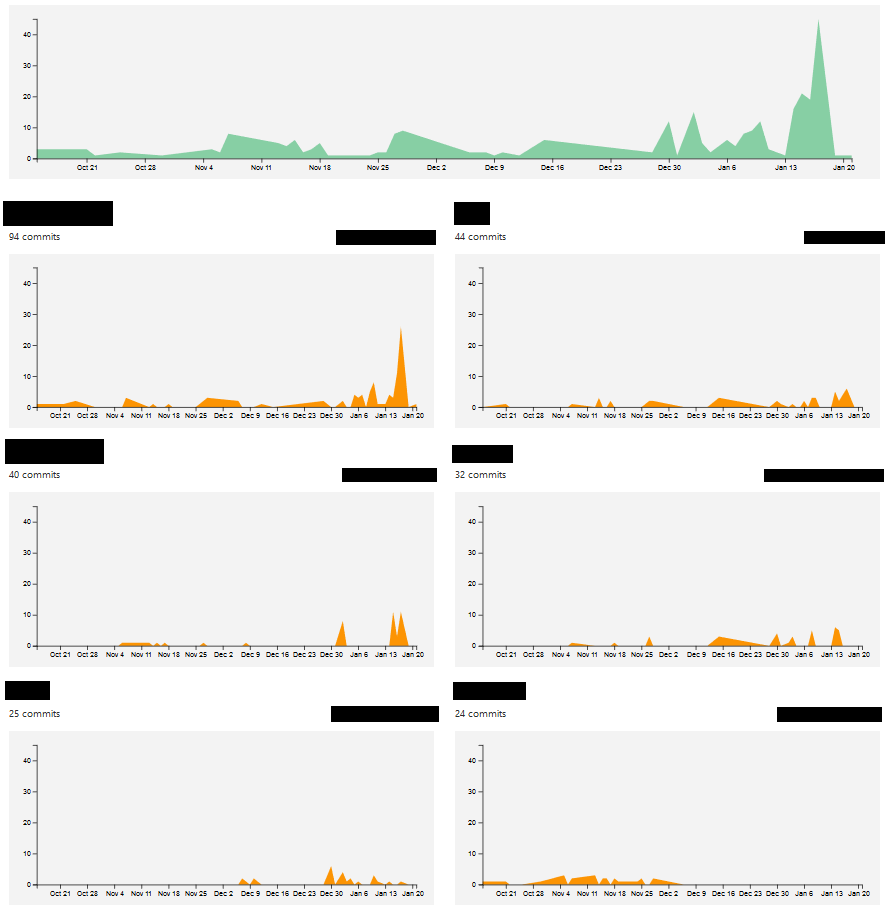
\includegraphics[scale=0.4]{slike/aktivnost.PNG} %veličina slike u odnosu na originalnu datoteku i pozicija slike
			\centering
			\caption{Primjer slike s potpisom}
			\label{fig:promjene}
		\end{figure}
		
		\begin{figure}[H]
			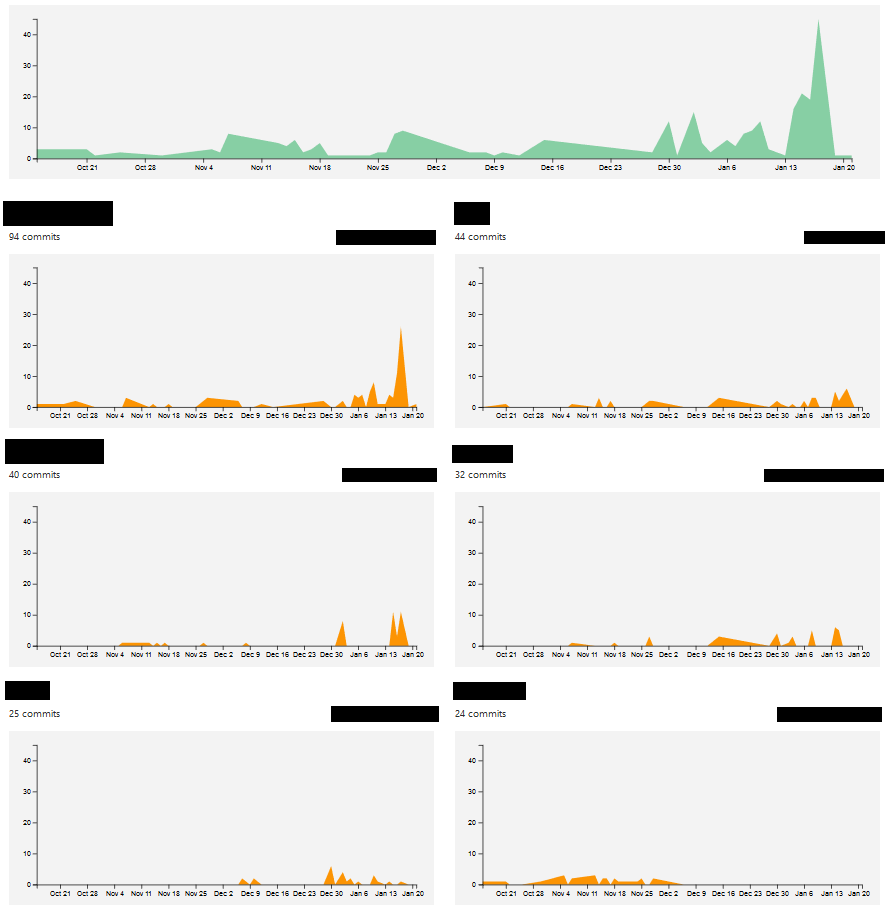
\includegraphics[width=\textwidth]{slike/aktivnost.PNG} %veličina u odnosu na širinu linije
			\caption{Primjer slike s potpisom 2}
			\label{fig:promjene2} %label mora biti drugaciji za svaku sliku
		\end{figure}
		
		Referenciranje slike \ref{fig:promjene2} u tekstu.
		
		\eject
		
	